% These packages are optional, depending whether you want the features they provide.
% See the LaTeX Companion or other references for full information.
% !TEX TS-program = pdflatex
% !TEX encoding = UTF-8 Unicode

% This is a simple template for a LaTeX document using the "article" class.
% See "book", "report", "letter" for other types of document.

\documentclass[12pt]{article} % use larger type; default would be 10pt
\usepackage[T2A]{fontenc}
\usepackage[utf8]{inputenc} % set input encoding (not needed with XeLaTeX)
\usepackage[russian]{babel}
%%% Examples of Article customizations
% These packages are optional, depending whether you want the features they provide.
% See the LaTeX Companion or other references for full information.

%%% PAGE DIMENSIONS
\usepackage{geometry}

\usepackage{fancyhdr} 
\geometry{a4paper} % or letterpaper (US) or a5paper or....
% \geometry{margin=2in} % for example, change the margins to 2 inches all round
% \geometry{landscape} % set up the page for landscape
%   read geometry.pdf for detailed page layout information
\usepackage{sectsty}
\usepackage{graphicx} % support the \includegraphics command and options
\usepackage{mathtext}
\usepackage{amsmath}
\usepackage{amsfonts}
% \usepackage[indentfill]{indentskip} % Activate to begin indentagraphs with an empty line rather than an indent
\usepackage{biblatex}
\usepackage{hyperref}
\hypersetup{
  colorlinks=true,
  linkcolor=blue,
  urlcolor=green
}
%%% END Article customizations

%%% The "real" document content comes below...
\usepackage{setspace}
\usepackage[section]{minted}

%%% ToC (table of contents) APPEARANCE
\usepackage[nottoc,notlof,notlot]{tocbibind} % Put the bibliography in the ToC
\usepackage[titles,subfigure]{tocloft} % Alter the style of the Table of Contents

%\date{} % Activate to display a given date or no date (if empty),
         % otherwise the current date is printed 
\usepackage{physics}
\usepackage{float}
\begin{titlepage}
	\thispagestyle{empty}
	\begin{center}
	\large{МИНОБРНАУКИ РОССИИ}\\
	\footnotesize{ФЕДЕРАЛЬНОЕ ГОСУДАРСТВЕННОЕ БЮДЖЕТНОE ОБРАЗОВАТЕЛЬНОЕ УЧРЕЖДЕНИЕ}\\ 
	\footnotesize{ВЫСШЕГО ПРОФЕССИОНАЛЬНОГО ОБРАЗОВАНИЯ}\\ 
	\small{\textbf{«САНКТ-ПЕТЕРБУРГСКИЙ ГОСУДАРСТВЕННЫЙ ПОЛИТЕХНИЧЕСКИЙ УНИВЕРСИТЕТ ПЕТРА ВЕЛИКОГО»}}\\
	\hfill \break
	\normalsize{Институт компьютерных наук и технологий}\\
	\hfill \break
	\normalsize{Высшая школа искусственного интеллекта}\\
	\hfill\break
	\begin{center}
		\normalsize{Дисциплина: \\ПРОГРАММИРОВАНИЕ МИКРОКОНТРОЛЛЕРОВ}
	\end{center}
	\hfill \break
	\hfill \break
	\large{ОТЧЕТ}\\
	\large{По лабораторной работе №6}\\
	\medium{Тема: Управление аппаратными таймерами STM32F200}\\
	\hfill \break
	\hfill \break
	\hfill \break
	\hfill \break
	\hfill \break
	\hfill \break
\end{center}	

\normalsize{ 
	\begin{tabular}{ccc}
		Обучающийся &  гр. 3530201/10001 & Нгуен Куок Дат \\\\
		Руководитель & \hrulefill 				&Вербова Наталья Михайловна\\\\
	\end{tabular}
}\\
\hfill \break
\hfill \break
\hfill \break
\hfill \break
\begin{center} Санкт-Петербург 2022 
\end{center}
\end{titlepage}
\usepackage{indentfirst}

\begin{document}
\begin{center}
\input{titlepage}
\end{center}
\doublespacing
\tableofcontents
\newpage
\section{Цель и постановка задачи}
\subsection{Цель работы}
Закрепить навыки работы с низкоуровневыми библиотеками и промежуточным программным обеспечением микроконтроллера. Ознакомится со способами управления аппаратными таймерами STM32F200. Ознакомиться с приемами отладки программ.

\subsection{Постановка задачи}

Разработать программу для микроконтроллера (МК) STM32F200, которая включает и выключает светодиоды: один при достижении содержимым таймера заданных значений, а
другой при достижении заданных значений содержимым программного счетчика.

\end{itemize}

\section{Выполнение задания}
\subsection{Коды программы}

\subsection{Измерения}
\subsubsection*{Опыт A}

\begin{figure}[H]
    \begin{subfigure}
        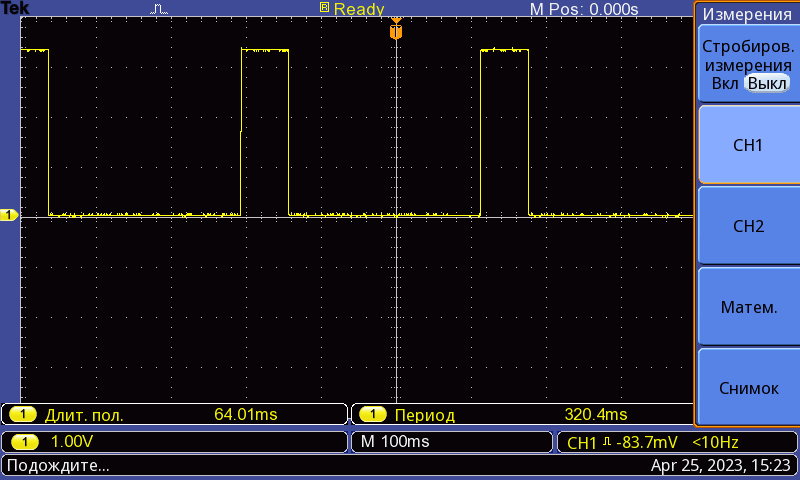
\includegraphics[width = 0.3\linewidth]{F:/git/micro/Lab6/report/20.png}	
    \end{subfigure}
    \hfill
    \begin{subfigure}
        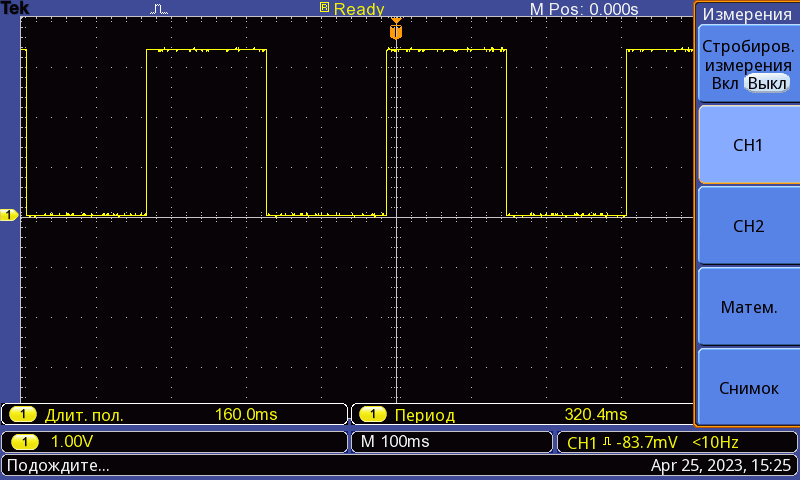
\includegraphics[width = 0.3\linewidth]{F:/git/micro/Lab6/report/50.png}	
    \end{subfigure}
    \hfill
    \begin{subfigure}
        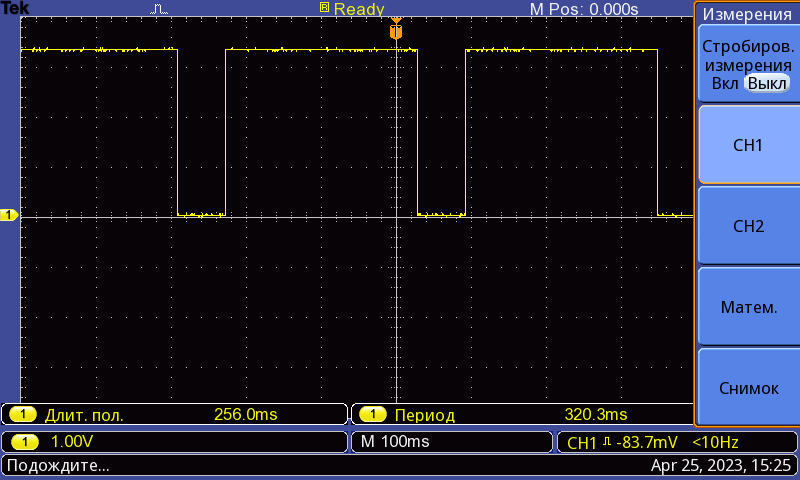
\includegraphics[width = 0.3\linewidth]{F:/git/micro/Lab6/report/80.png}	
    \end{subfigure}
    \caption{Вольны с разными заполнениями: 20\%, 50\%, 80\%}
\end{figure}


\subsubsection*{Опыт B,C}

\begin{figure}[H]
    \begin{subfigure}
        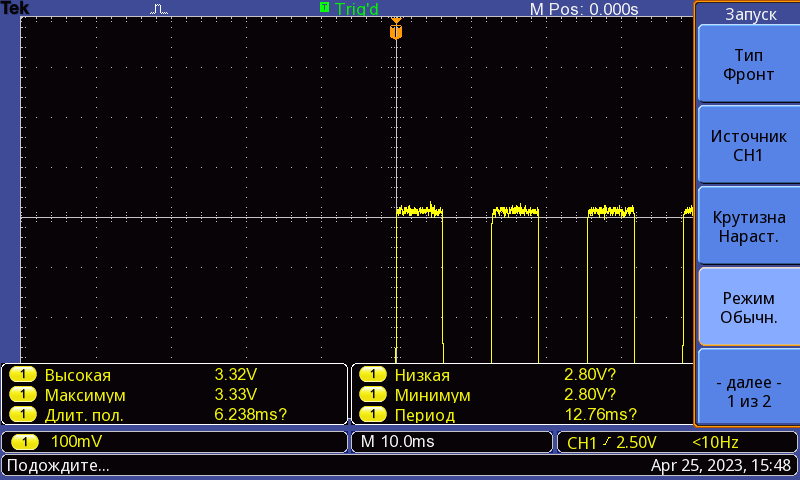
\includegraphics[width = 0.4\linewidth]{F:/git/micro/Lab6/report/high.png}	
    \end{subfigure}
    \hfill
    \begin{subfigure}
        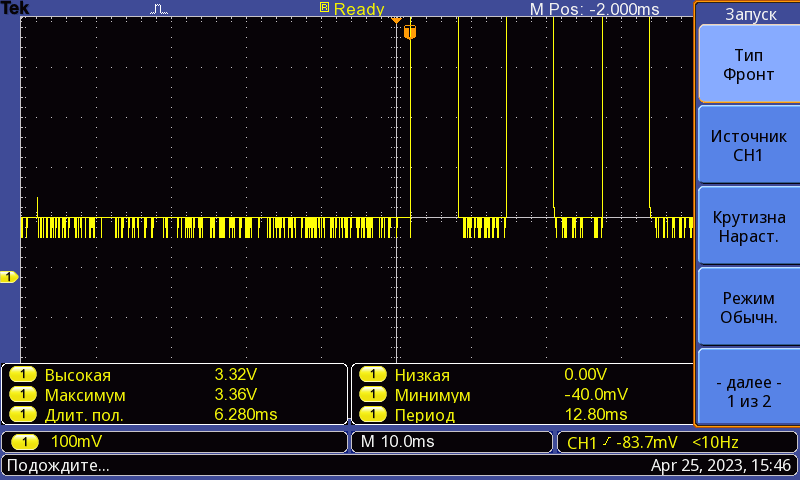
\includegraphics[width = 0.4\linewidth]{F:/git/micro/Lab6/report/low.png}	
    \end{subfigure}
    \caption{Верхние и нижние границы}
\end{figure}

\[
\begin{align}
    & U_\text{верх} = 3.32V \\
   &  U_\text{ниж} = 0.00V \\
&    U_\text{макс} = 3.36V \\
  &  U_\text{мин} = -40.0mV \\
    &\text{Перегулирование:}\\
    &U_\text{пол} = 1,2\%\\
    &U_\text{отр} = 1,2\%\\
 \end{align}
\]



\subsubsection*{Опыт D,E}

\begin{figure}[H]
    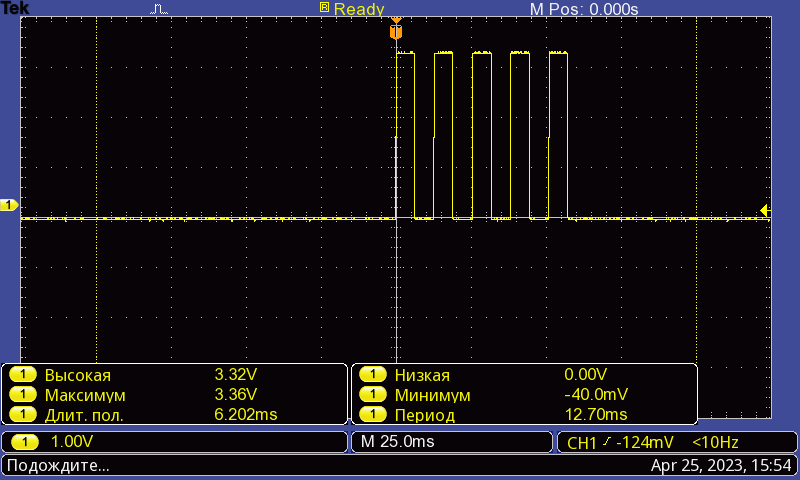
\includegraphics[width = 0.9\linewidth]{F:/git/micro/Lab6/report/group.png}	
\end{figure}
\[ 
\begin{align}
   & \#\text{положительных импульсов} = 5\\
    &\#\text{отрицательных импульсов} = 5\\
    &\text{Ширина пачки импульсов} = 6.2*5 = 31ms\\
\end{align}
\]

\end{document}